\chapter{Topological HLT Development at $\sqrt{s}=13 \TeV$}
\label{ch:hlt13TeV}

To target a broad range of new physics possibilities, we designed four different
types of triggers for use at $\sqrt{s}=13\TeV$:
\begin{itemize}
\item Dijet razor trigger with hyperbolic \MR and \Rtwo requirements targetting the squark pair production topology;
\item Quadjet razor trigger with hyperbolic \MR and \Rtwo requirements
  targetting top-squark or gluino pair production topologies;
\item High-\Rtwo trigger targetting dijet+invisible topologies with
  large transverse momentum imbalance; and
\item Razor $\PH(\bbbar)$ trigger targetting production of
  $\PH(\bbbar)+\mathrm{jet}+\mathrm{invisible}$ with some transverse momentum imbalance.
\end{itemize}

The dijet and quadjet razor triggers are broadly motivated by SUSY pair
production and represent an update and incremental improvement of the razor triggers
used in previous searches at $\sqrt{s}=8\TeV$~\cite{razor8TeV}. Both
sets of triggers are based on hyperbolic thresholds in the $(\MR,\Rtwo)$
plane, with the 2015 updated thresholds shown in
Fig~\ref{fig:hyperbolic}. The 2015 hyperbolic contours follow the
iso-probability contours derived from the background-only fit to the MultiJet category
in the 8\TeV razor search performed using 2012 data. This implies
these hyperbolic contours efficiently reject background, while
maintaining a large acceptance for SUSY signal models with large
characteristic mass scale $M_{\Delta}\gtrsim 500 \GeV$ and sufficient
transverse momentum imbalance. Another update is that the 13 \TeV razor triggers are based on PF-reconstructed objects rather
than Calo jets and muons, which means the online $\Rtwo$ variable is
much more correlated with the offline $\Rtwo$ variable, which is also
PF-based. This leads to an improved trigger efficiency for 2015, shown
in Fig.~\ref{fig:turnons}.

\begin{figure}[htb!]
\centering
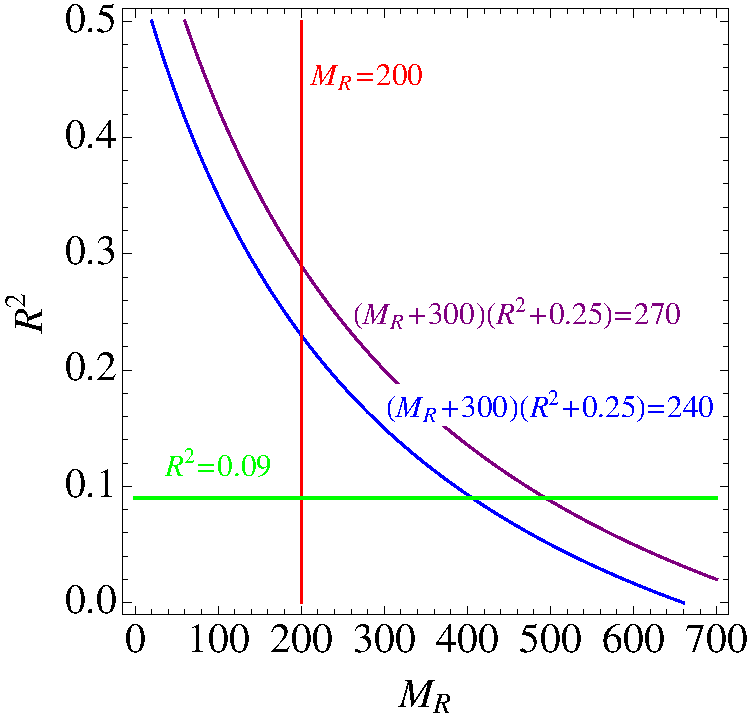
\includegraphics[width=0.49\textwidth]{figs/hlt13TeV/HLTRsqMR.pdf}
\caption{\label{fig:hyperbolic} Hyperbolic and baseline thresholds in
  \Rtwo and \MR used in the dijet and quadjet razor triggers.}
\end{figure}

\begin{figure}[ht!]
\centering
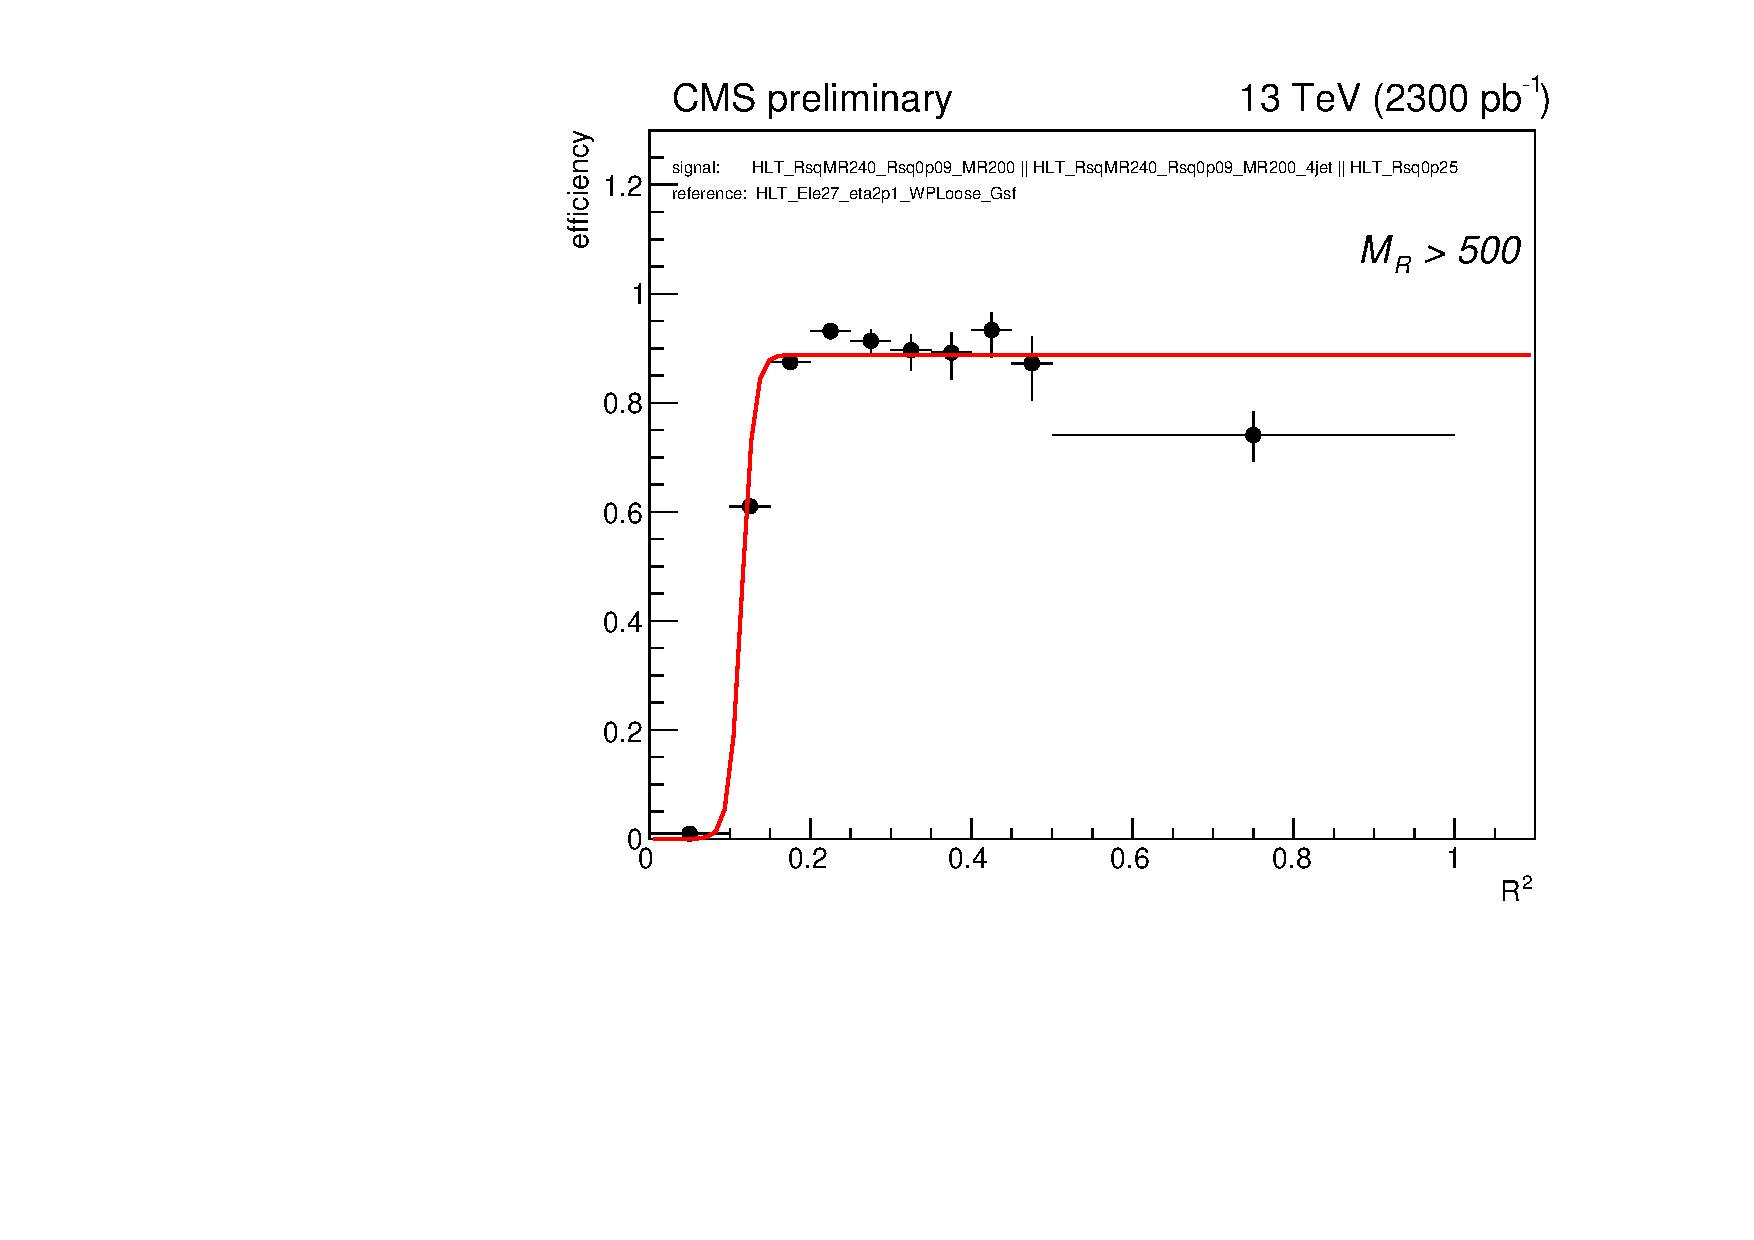
\includegraphics[width=0.45\textwidth]{figs/hlt13TeV/turnons_2015_no100GeVmuons/HLT_RsqMR240_Rsq0p09_MR200_HLT_RsqMR240_Rsq0p09_MR200_4jet_HLT_Rsq0p25_HLT_Ele27_eta2p1_WPLoose_Gsf_effRsq_MR500.pdf}
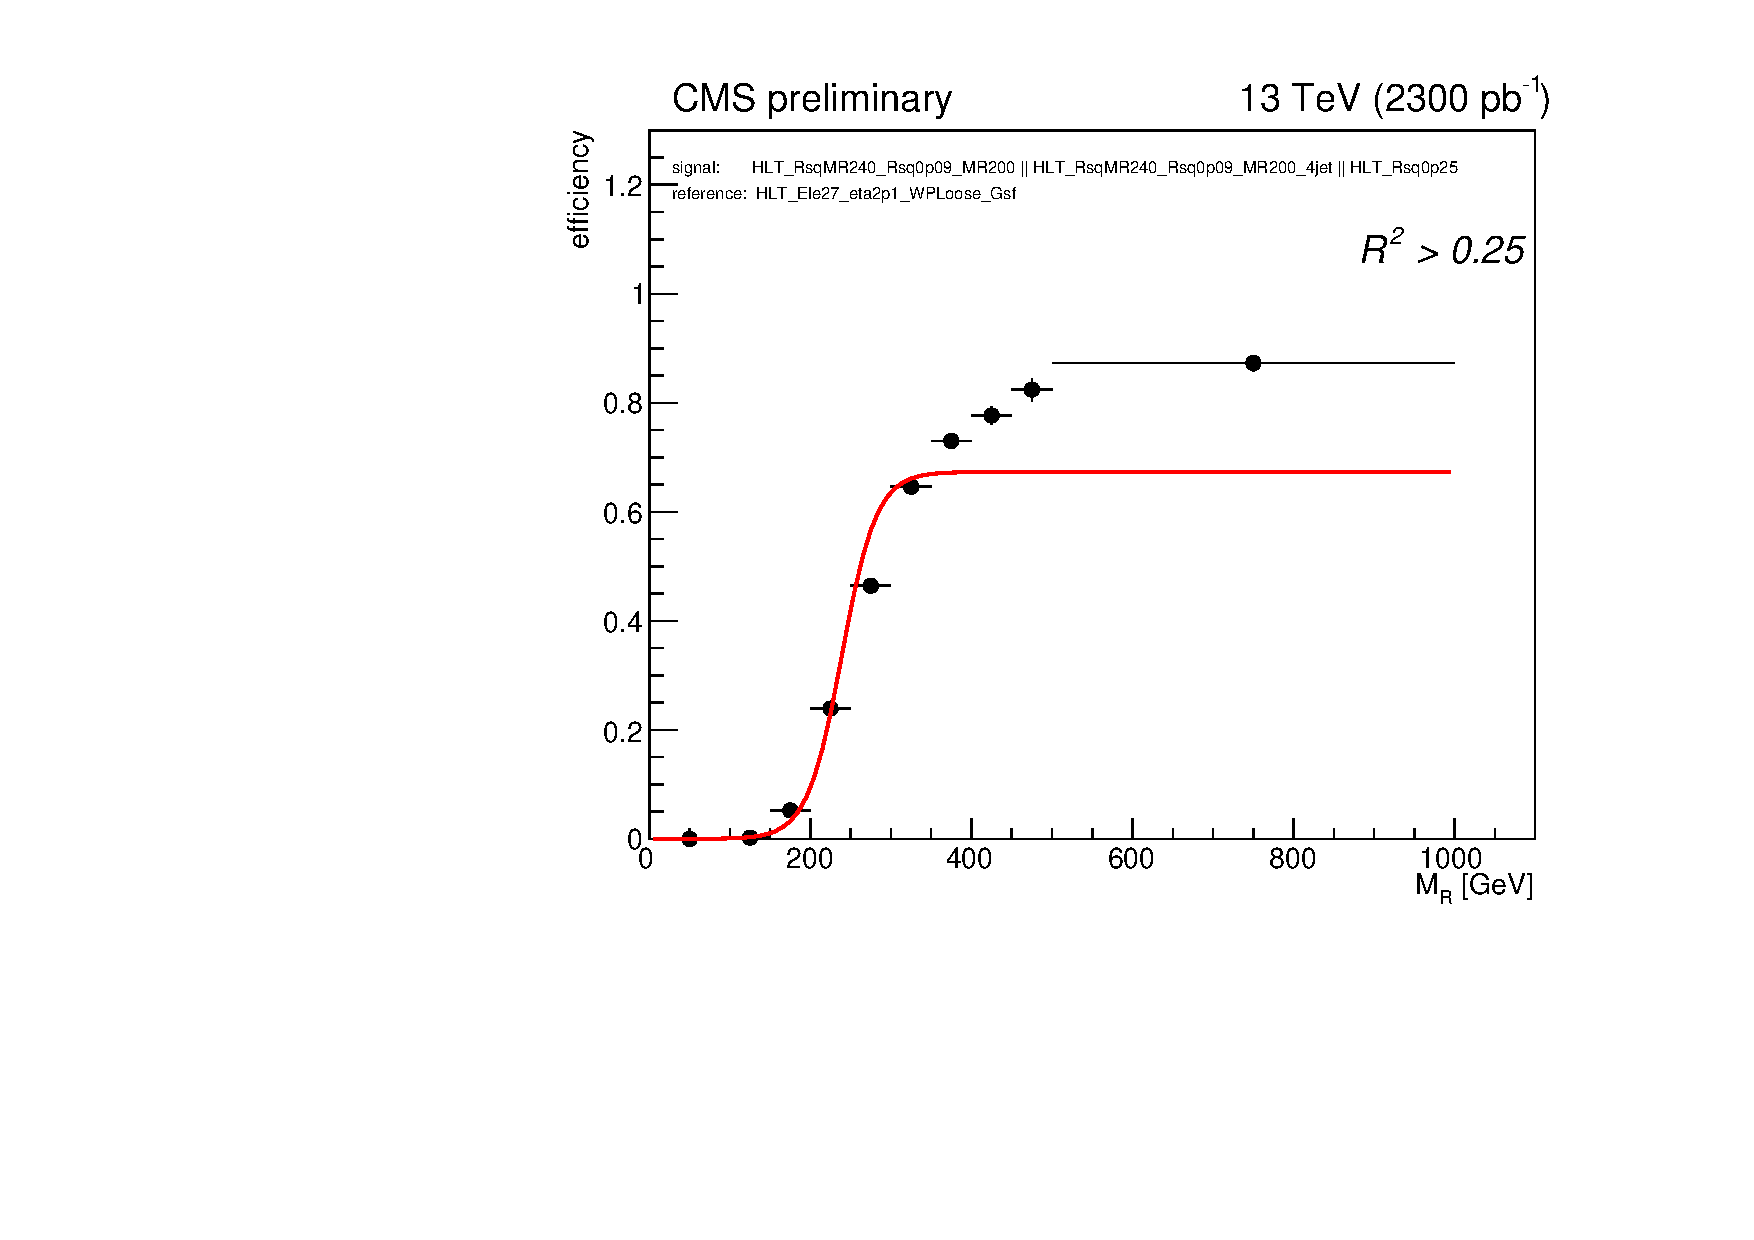
\includegraphics[width=0.45\textwidth]{figs/hlt13TeV/turnons_2015_no100GeVmuons/HLT_RsqMR240_Rsq0p09_MR200_HLT_RsqMR240_Rsq0p09_MR200_4jet_HLT_Rsq0p25_HLT_Ele27_eta2p1_WPLoose_Gsf_effMR_Rsq0p25.pdf}\\
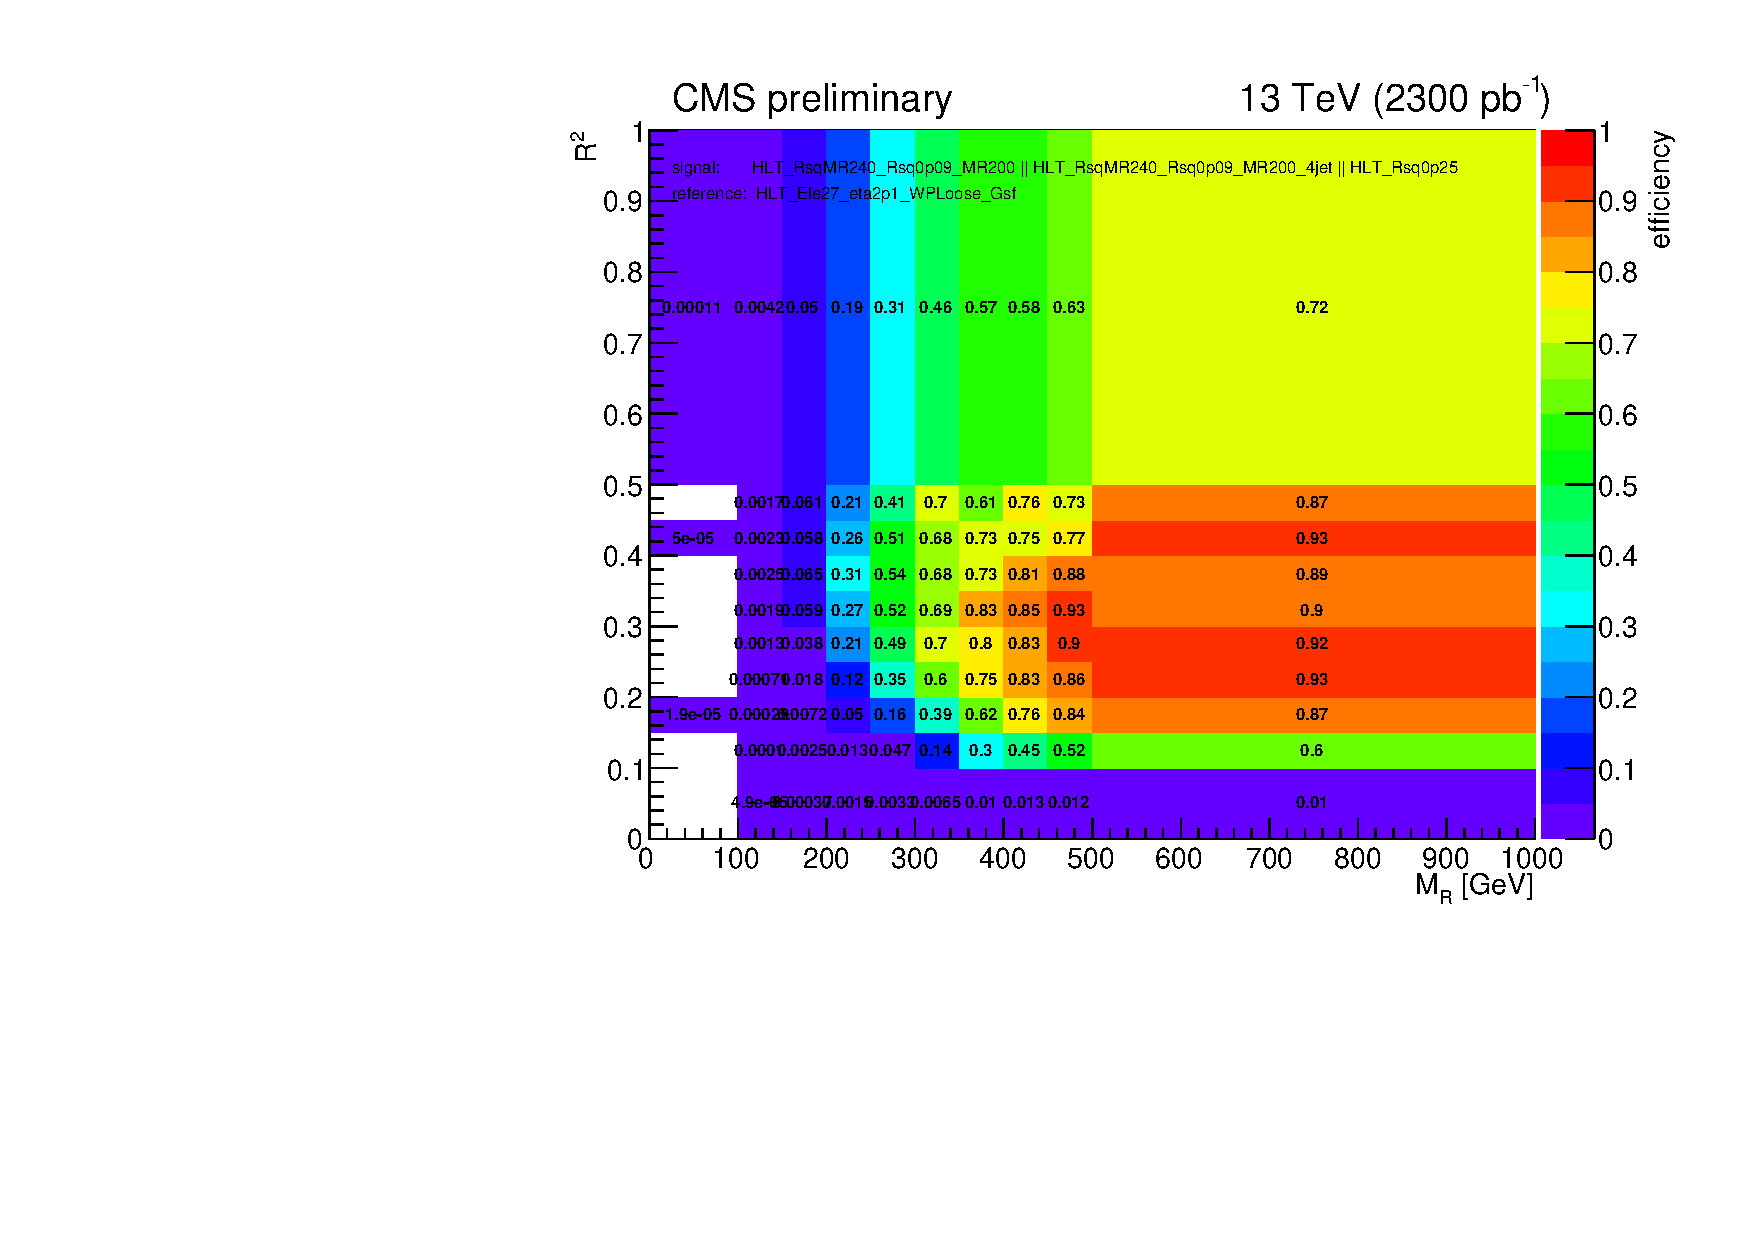
\includegraphics[width=0.45\textwidth]{figs/hlt13TeV/turnons_2015_no100GeVmuons/HLT_RsqMR240_Rsq0p09_MR200_HLT_RsqMR240_Rsq0p09_MR200_4jet_HLT_Rsq0p25_HLT_Ele27_eta2p1_WPLoose_Gsf_eff2D.pdf}
\caption{\label{fig:turnons} Trigger efficiencies as measured using a
  data sample of single-electron events for $\Rtwo$ (top
  left), $\MR$ (top right), and in the $(\MR,\Rtwo)$ plane (bottom).}
\end{figure}

The high-\Rtwo trigger is motivated by the search for the direct
production of dark matter (DM) particles at the
LHC~\cite{Khachatryan:2016reg}.  DM particles themselves
would not leave a detectable signal in the detector, but if
they were produced in association with high-energy quarks or gluons,
they could produce signatures with jets and transverse
momentum imbalance. The traditional approach, employed by both CMS and
ATLAS, is to search in events with one high-$\pt$ jet and large $\MET$
(so-called monojet searches)~\cite{Aad:2011xw,Chatrchyan:2012me}. A complementary
approach is to search in events with at least two jets passing a looser
event selection using the razor variables. The sensitivity of these variables to direct DM production was
suggested in Ref.~\cite{Fox:2012ee}, and the search carried out by CMS
demonstrates that the resulting sensitivity is comparable to that of
monojet searches~\cite{Fox:2012ee,Papucci:2014iwa,Khachatryan:2016reg}.
The hallmark of many direct DM production models in the razor plane is an
almost-peaking behavior near $\Rtwo\gtrsim 0.8$ and an exponentially
falling $\MR$ distribution with no special structure. For this reason,
the high-\Rtwo trigger is designed with a threshold in \Rtwo but no
requirement on \MR to allow for greater DM signal acceptance.

Finally, the razor $\PH(\bbbar)$ trigger is motivated by an
excess observed by CMS in events with a $\PH
(\Pgg\Pgg)$ plus at least one extra jet~\cite{RazorHgaga}. The excess,
corresponding to a local significance of
$2.9\sigma$, consists of five events observed with $400\GeV<\MR<1400
\GeV$,  $\Rtwo>0.05$, and $m_{\Pgg\Pgg}$ consisent with $m_{h^0}= 125
\GeV$ in a high-resolution diphoton category, compared to less than one
expected background event. The general idea is to search for a similar
signature in the $\PH\to\bbbar$ channel, which comes with a larger
signal yield (90,000 times more assuming SM Higgs branching ratios),
but a much larger background, resulting in a considerably worse
signal-to-background ratio. To this end, the trigger
requirements of three jets, two \cPqb-jets, $\MR>300
\GeV$,  $\Rtwo>0.02$, and $m_{\bbbar}$ roughly consisent with $m_{h^0}= 125
\GeV$ are chosen to (a) maintain signal acceptance based on the observed
features, (b) accept additional events outside of $m_{h^0}$ window
to permit a robust background estimation based on a fit, and (c)
limit the rate and average CPU time of the trigger to an acceptable level.
%, reduced to $1.6\sigma$ after the LEE.

\section{HLT Path Design}

The design of the four main HLT paths in terms of producers (in
purple) and filters (in blue) is shown
in Fig.~\ref{fig:HLTdesign}. The first step is always a filter, which
rejects events with no hadronic activity above a certain threshold reconstructed by the L1 trigger.
As detailed in Sec.~\ref{sec:trigger}, there are two main technical
constraints an HLT path must satisfy: (a) the average CPU time required must be
small enough so that the entire HLT menu fits within the timing budget
 of $\sim160$ \unit{ms} and (b) the rate must
be small enough so that the entire HLT menu fits within the maximum
allowable rate  of $\sim1$ \unit{kHz}. To satisfy the timing
requirement, all the paths are outfitted with
calorimetric prefilters. The aim of these prefilters is to reject
events based only on information from the calorimeters, whose
reconstruction algorithms are much faster than the PF algorithm. In
other words, to keep the timing of the paths manageable, it is
necessary to limit the input rate to the PF algorithm. Thus, all four
triggers have prefilter based on calorimeter-based versions of the razor
variables.

\begin{figure}[ht!]
\centering
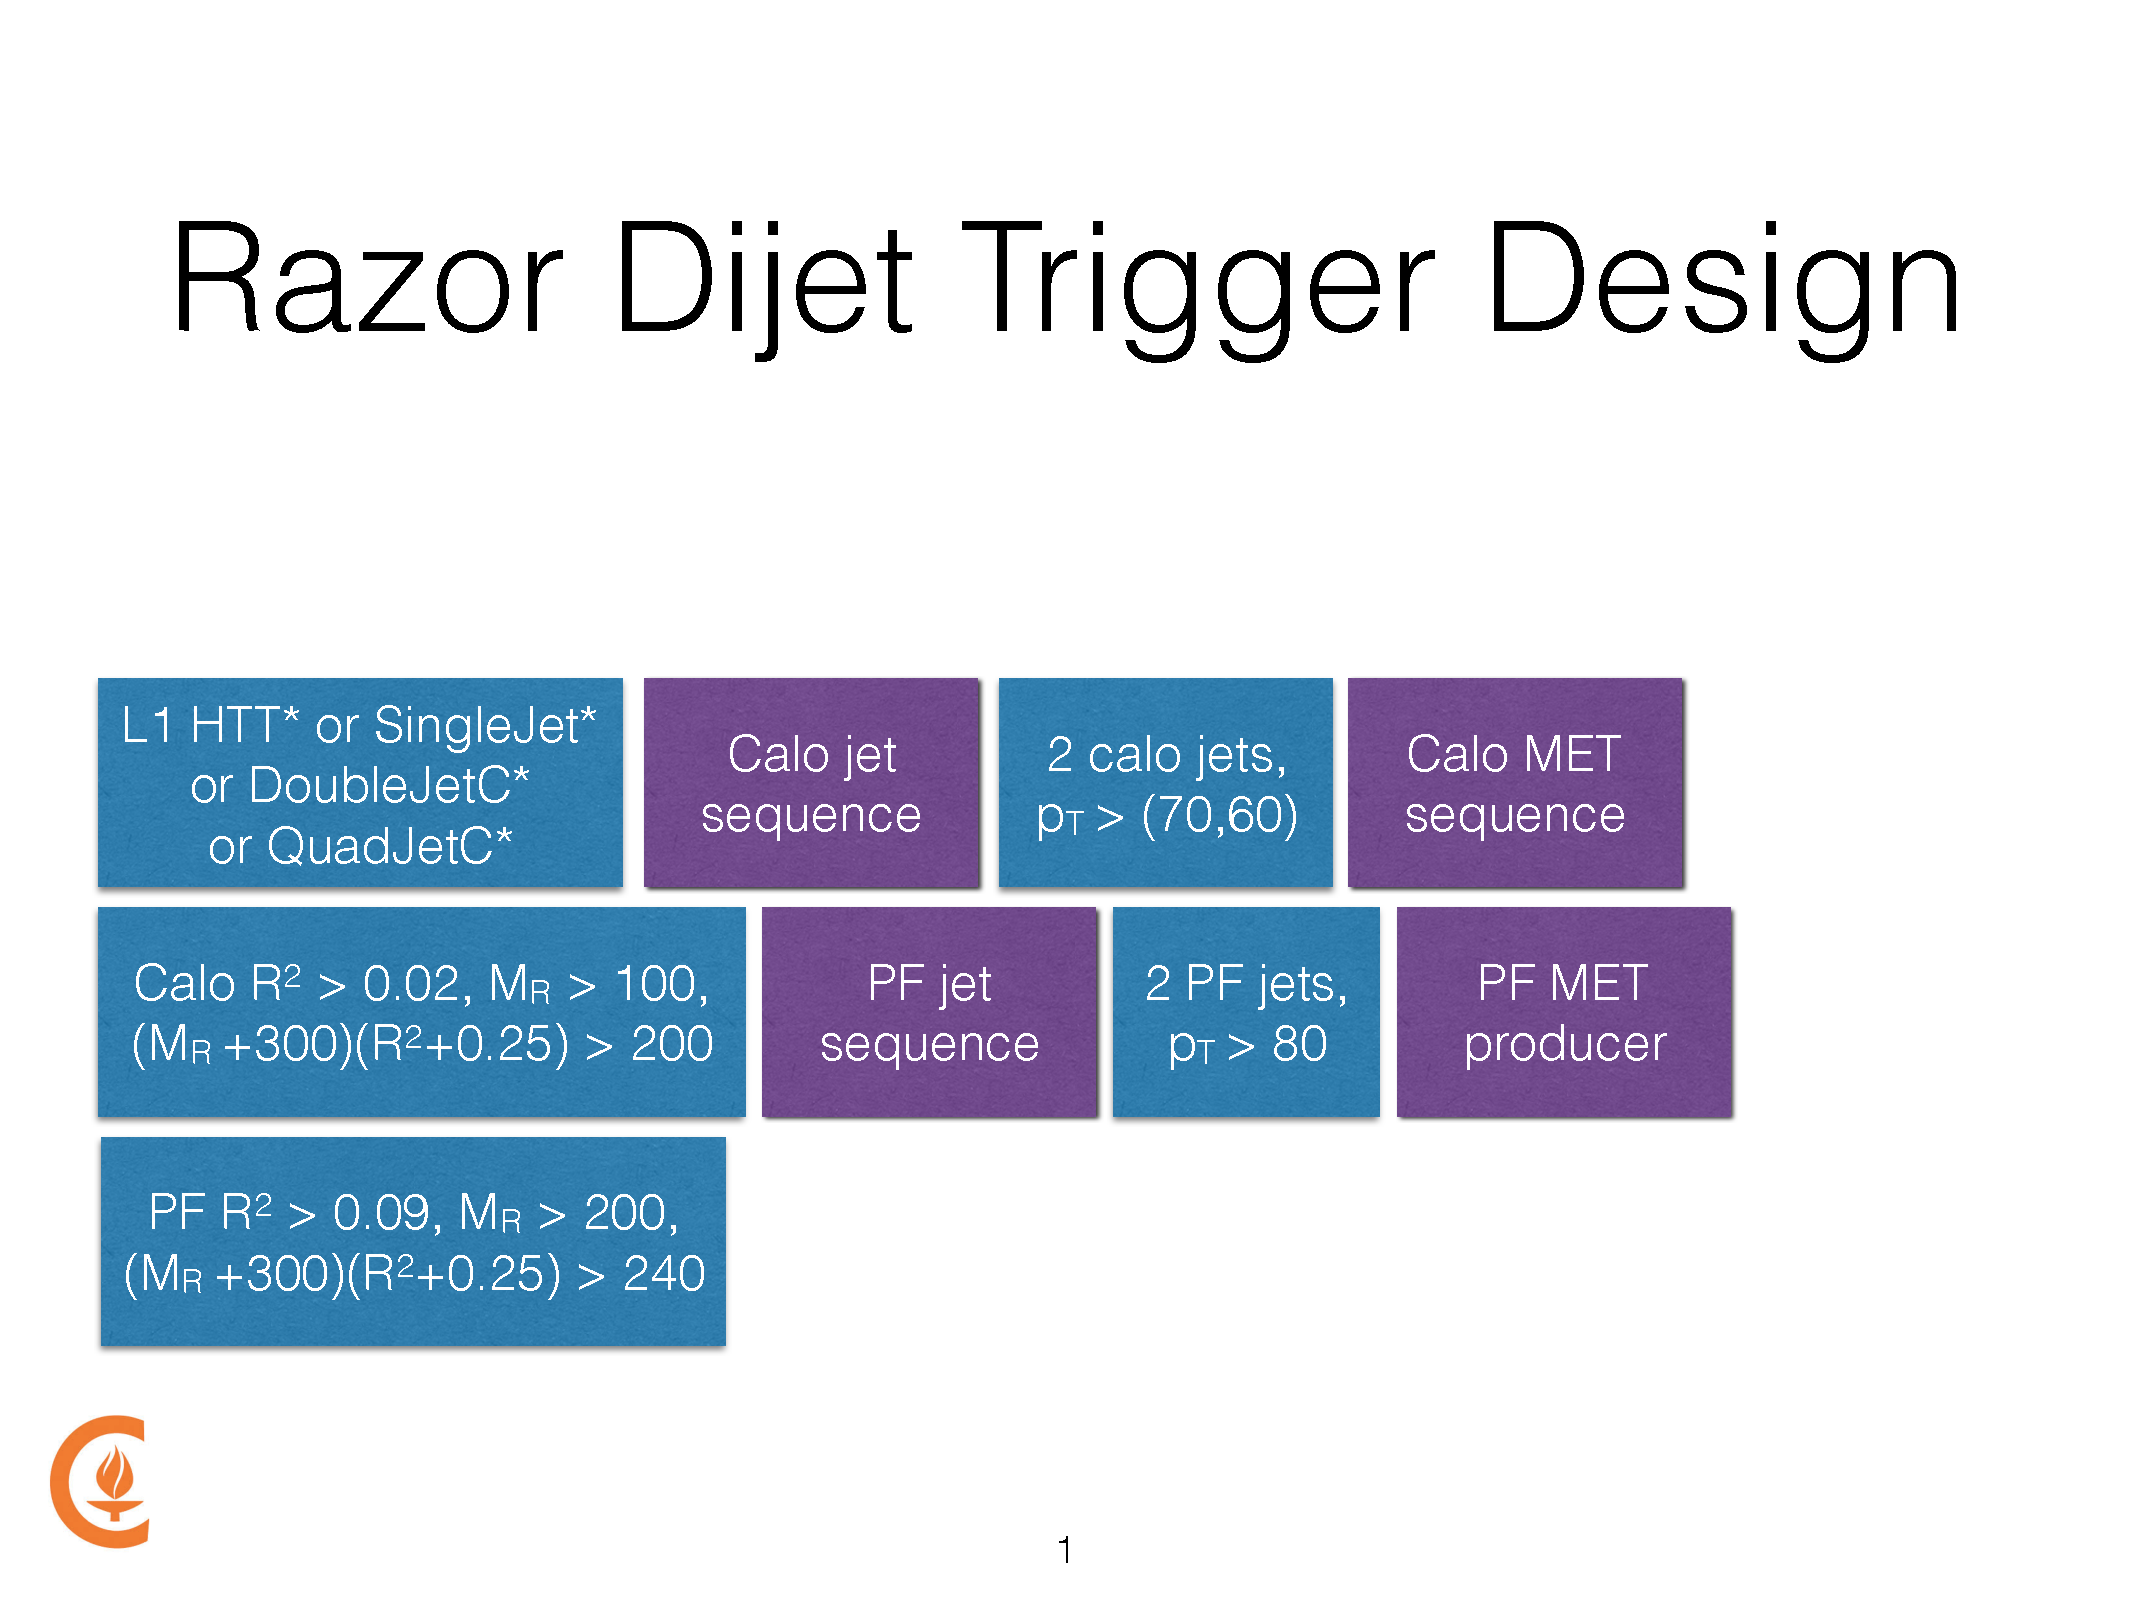
\includegraphics[width=0.8\textwidth,clip=true,viewport=0 110 1024
500]{figs/hlt13TeV/HLTDijetDesign.pdf}\\
(a) HLT\_RsqMR240\_Rsq0p09\_MR200 \\
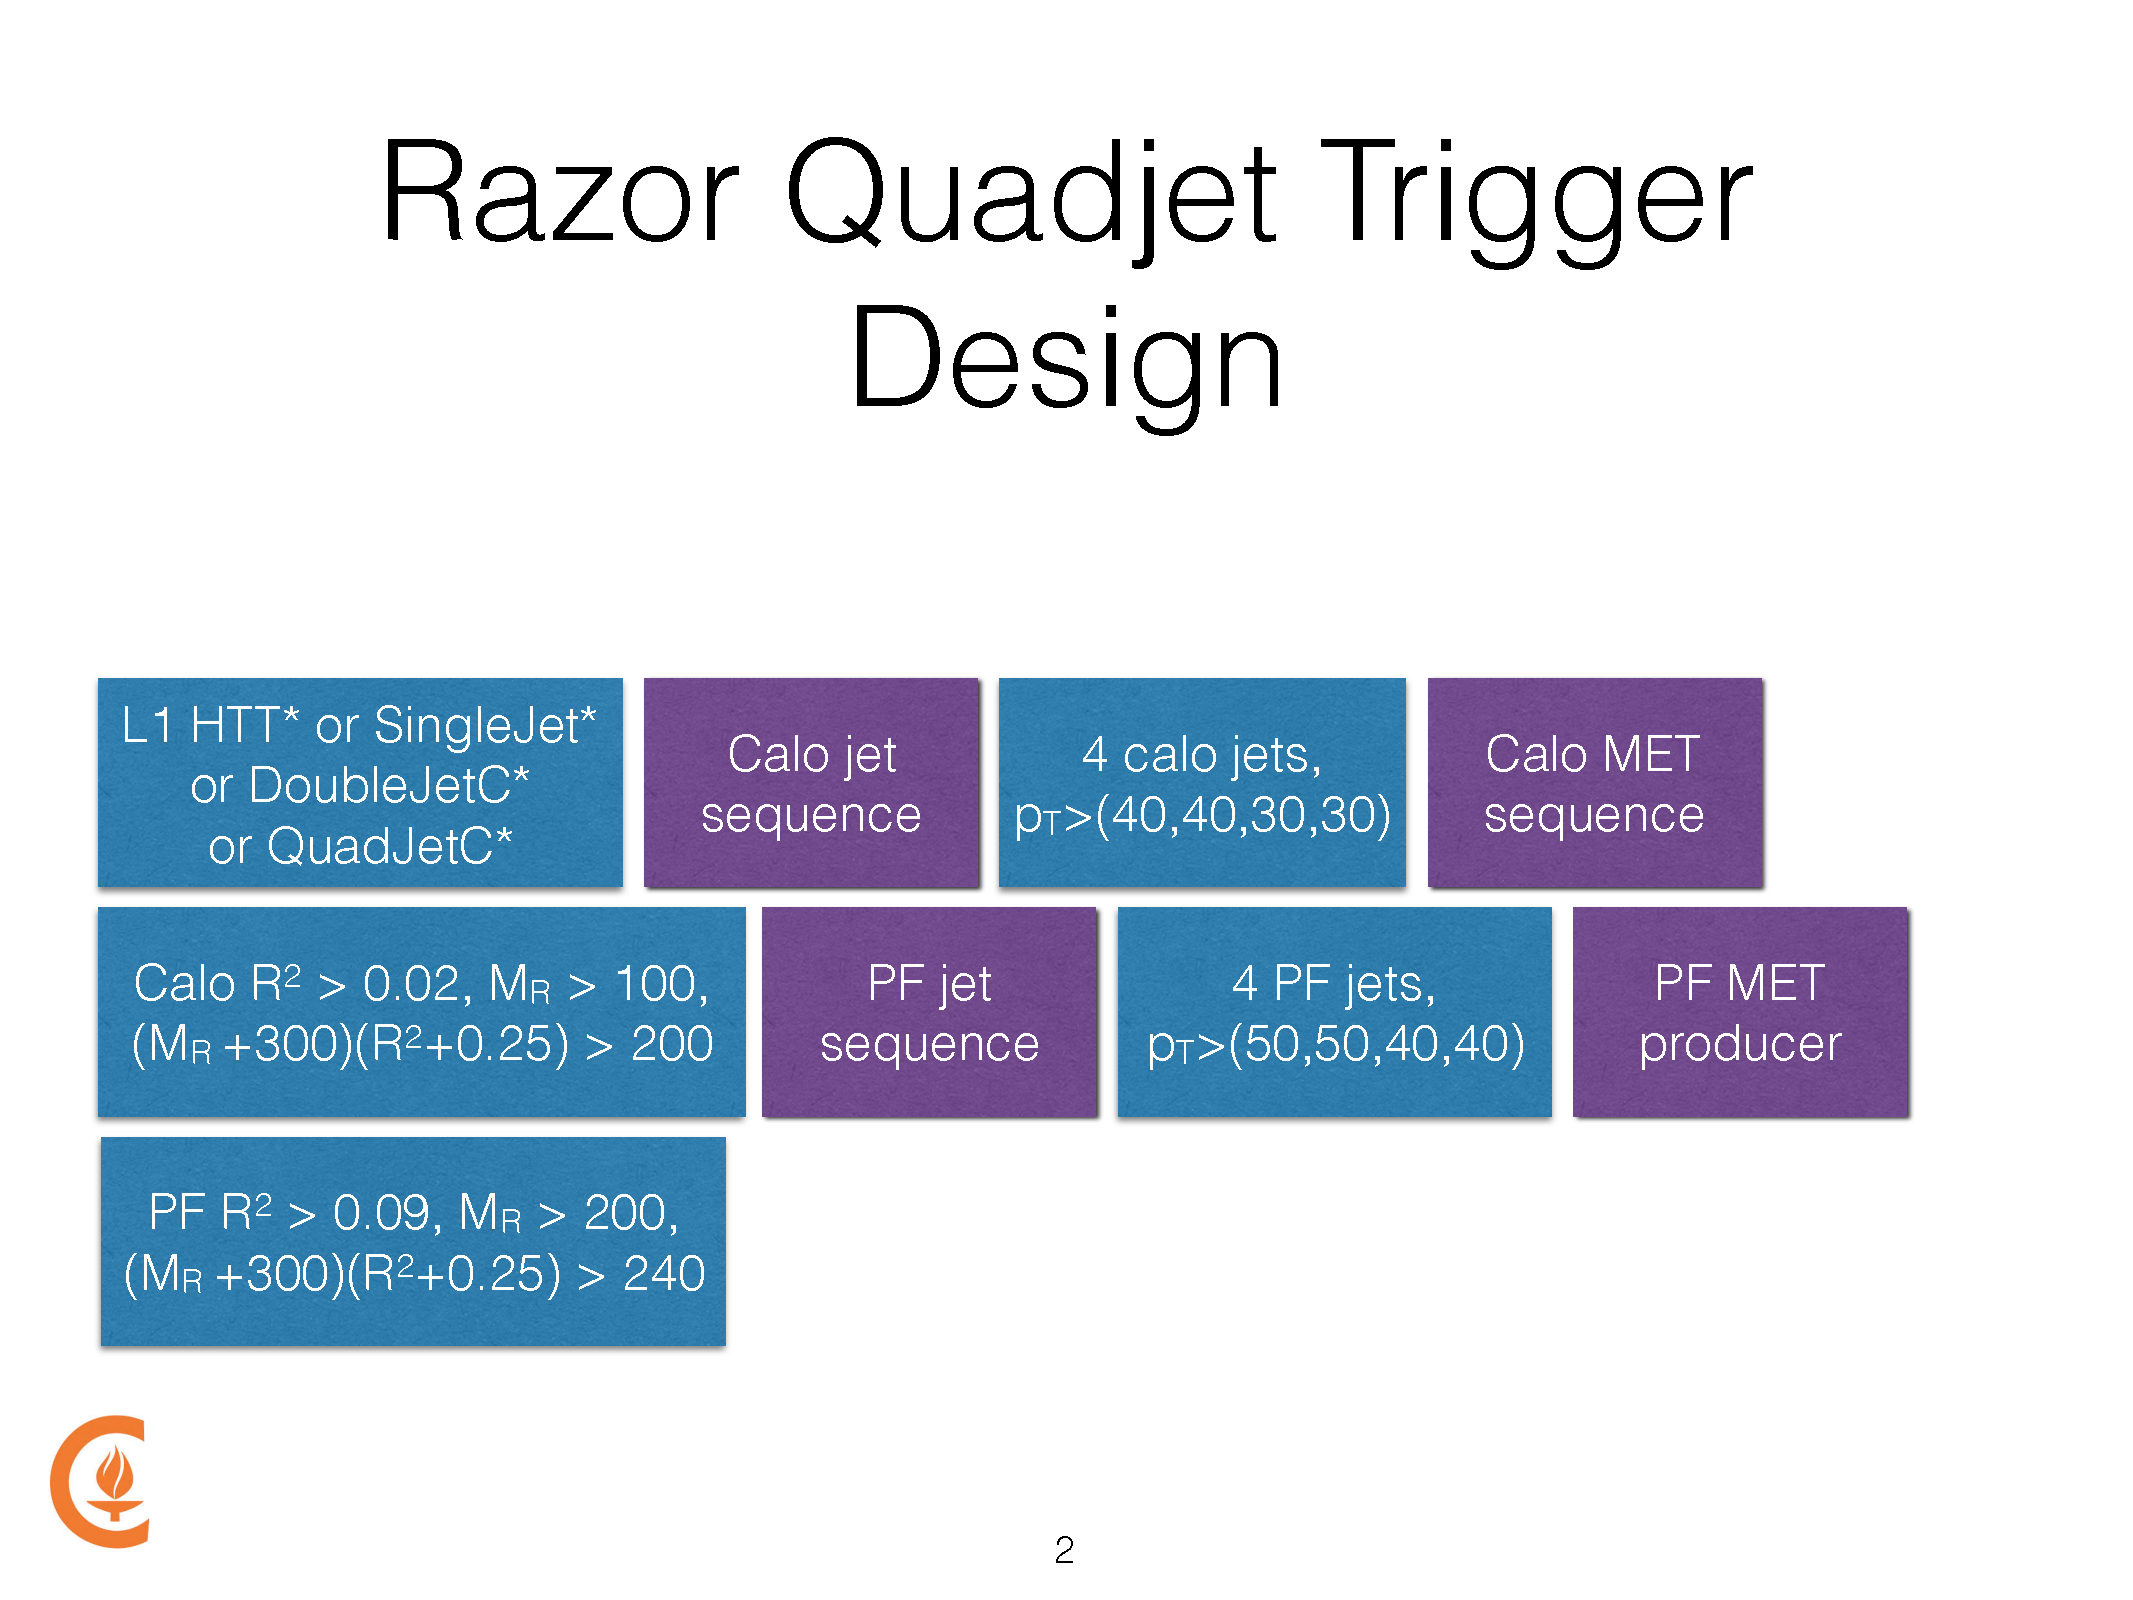
\includegraphics[width=0.8\textwidth,clip=true,viewport=0 110 1024
500]{figs/hlt13TeV/HLTQuadjetDesign.pdf}\\
(b) HLT\_RsqMR240\_Rsq0p09\_MR200\_4jet \\
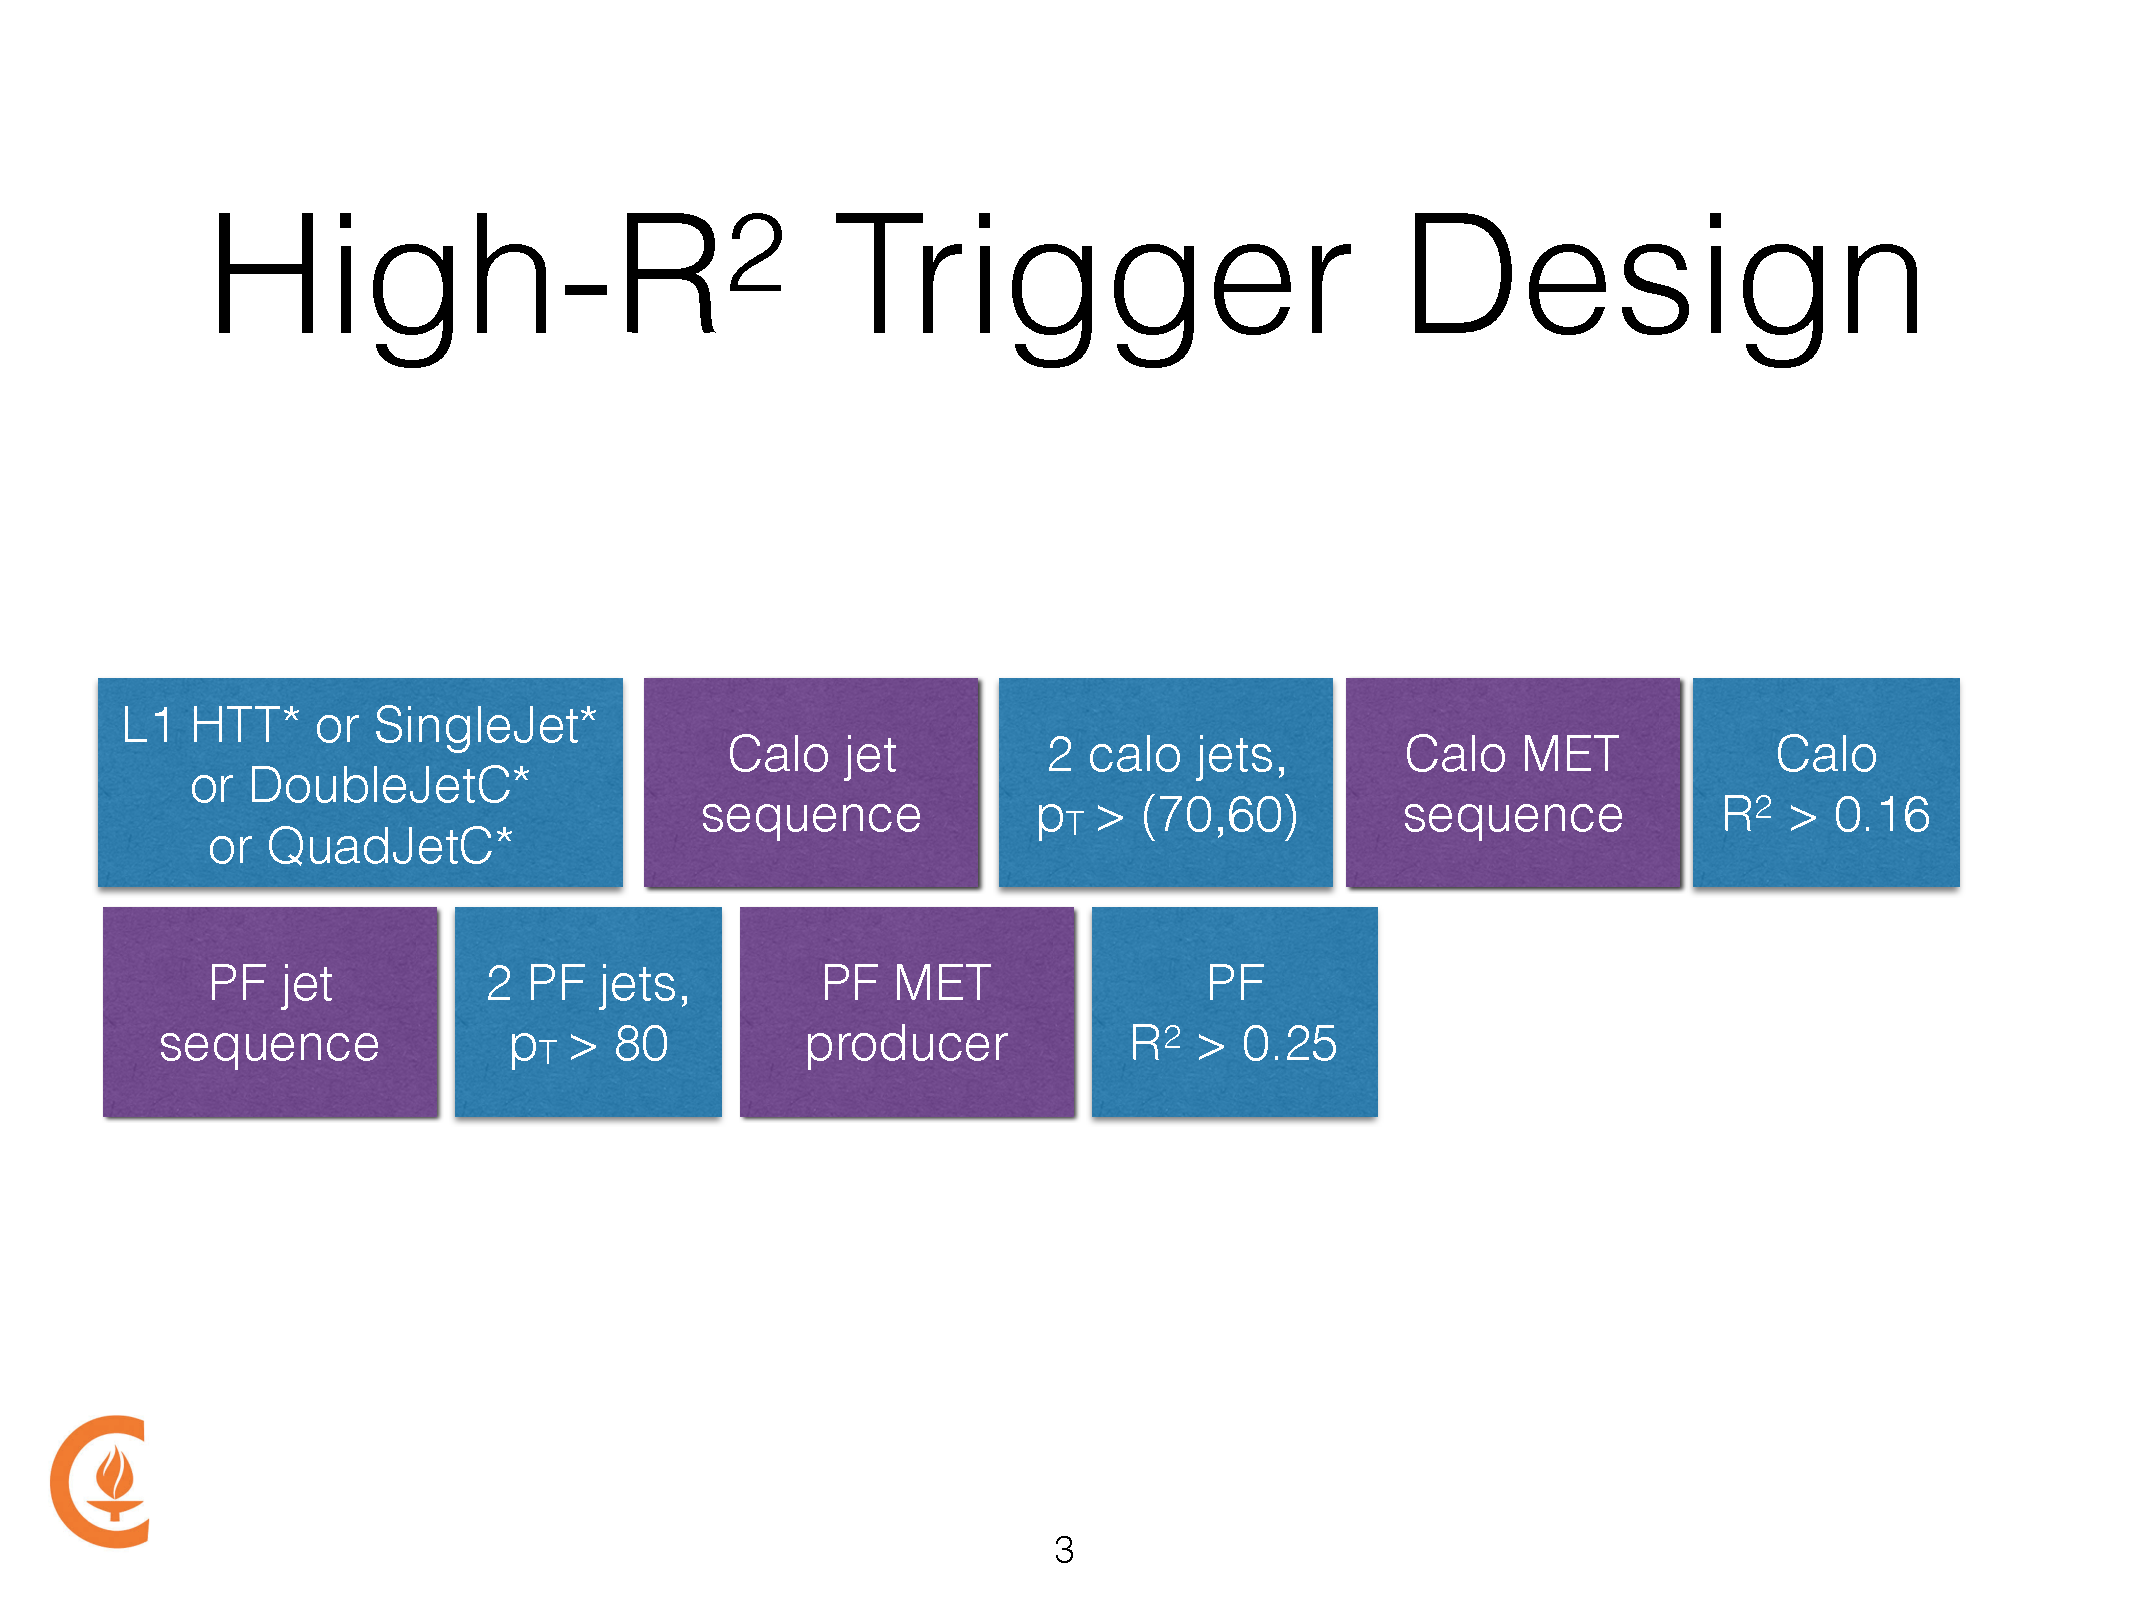
\includegraphics[width=0.8\textwidth,clip=true,viewport=0 220 1024
500]{figs/hlt13TeV/HLTR2Design.pdf}\\
(c) HLT\_Rsq0p25\\
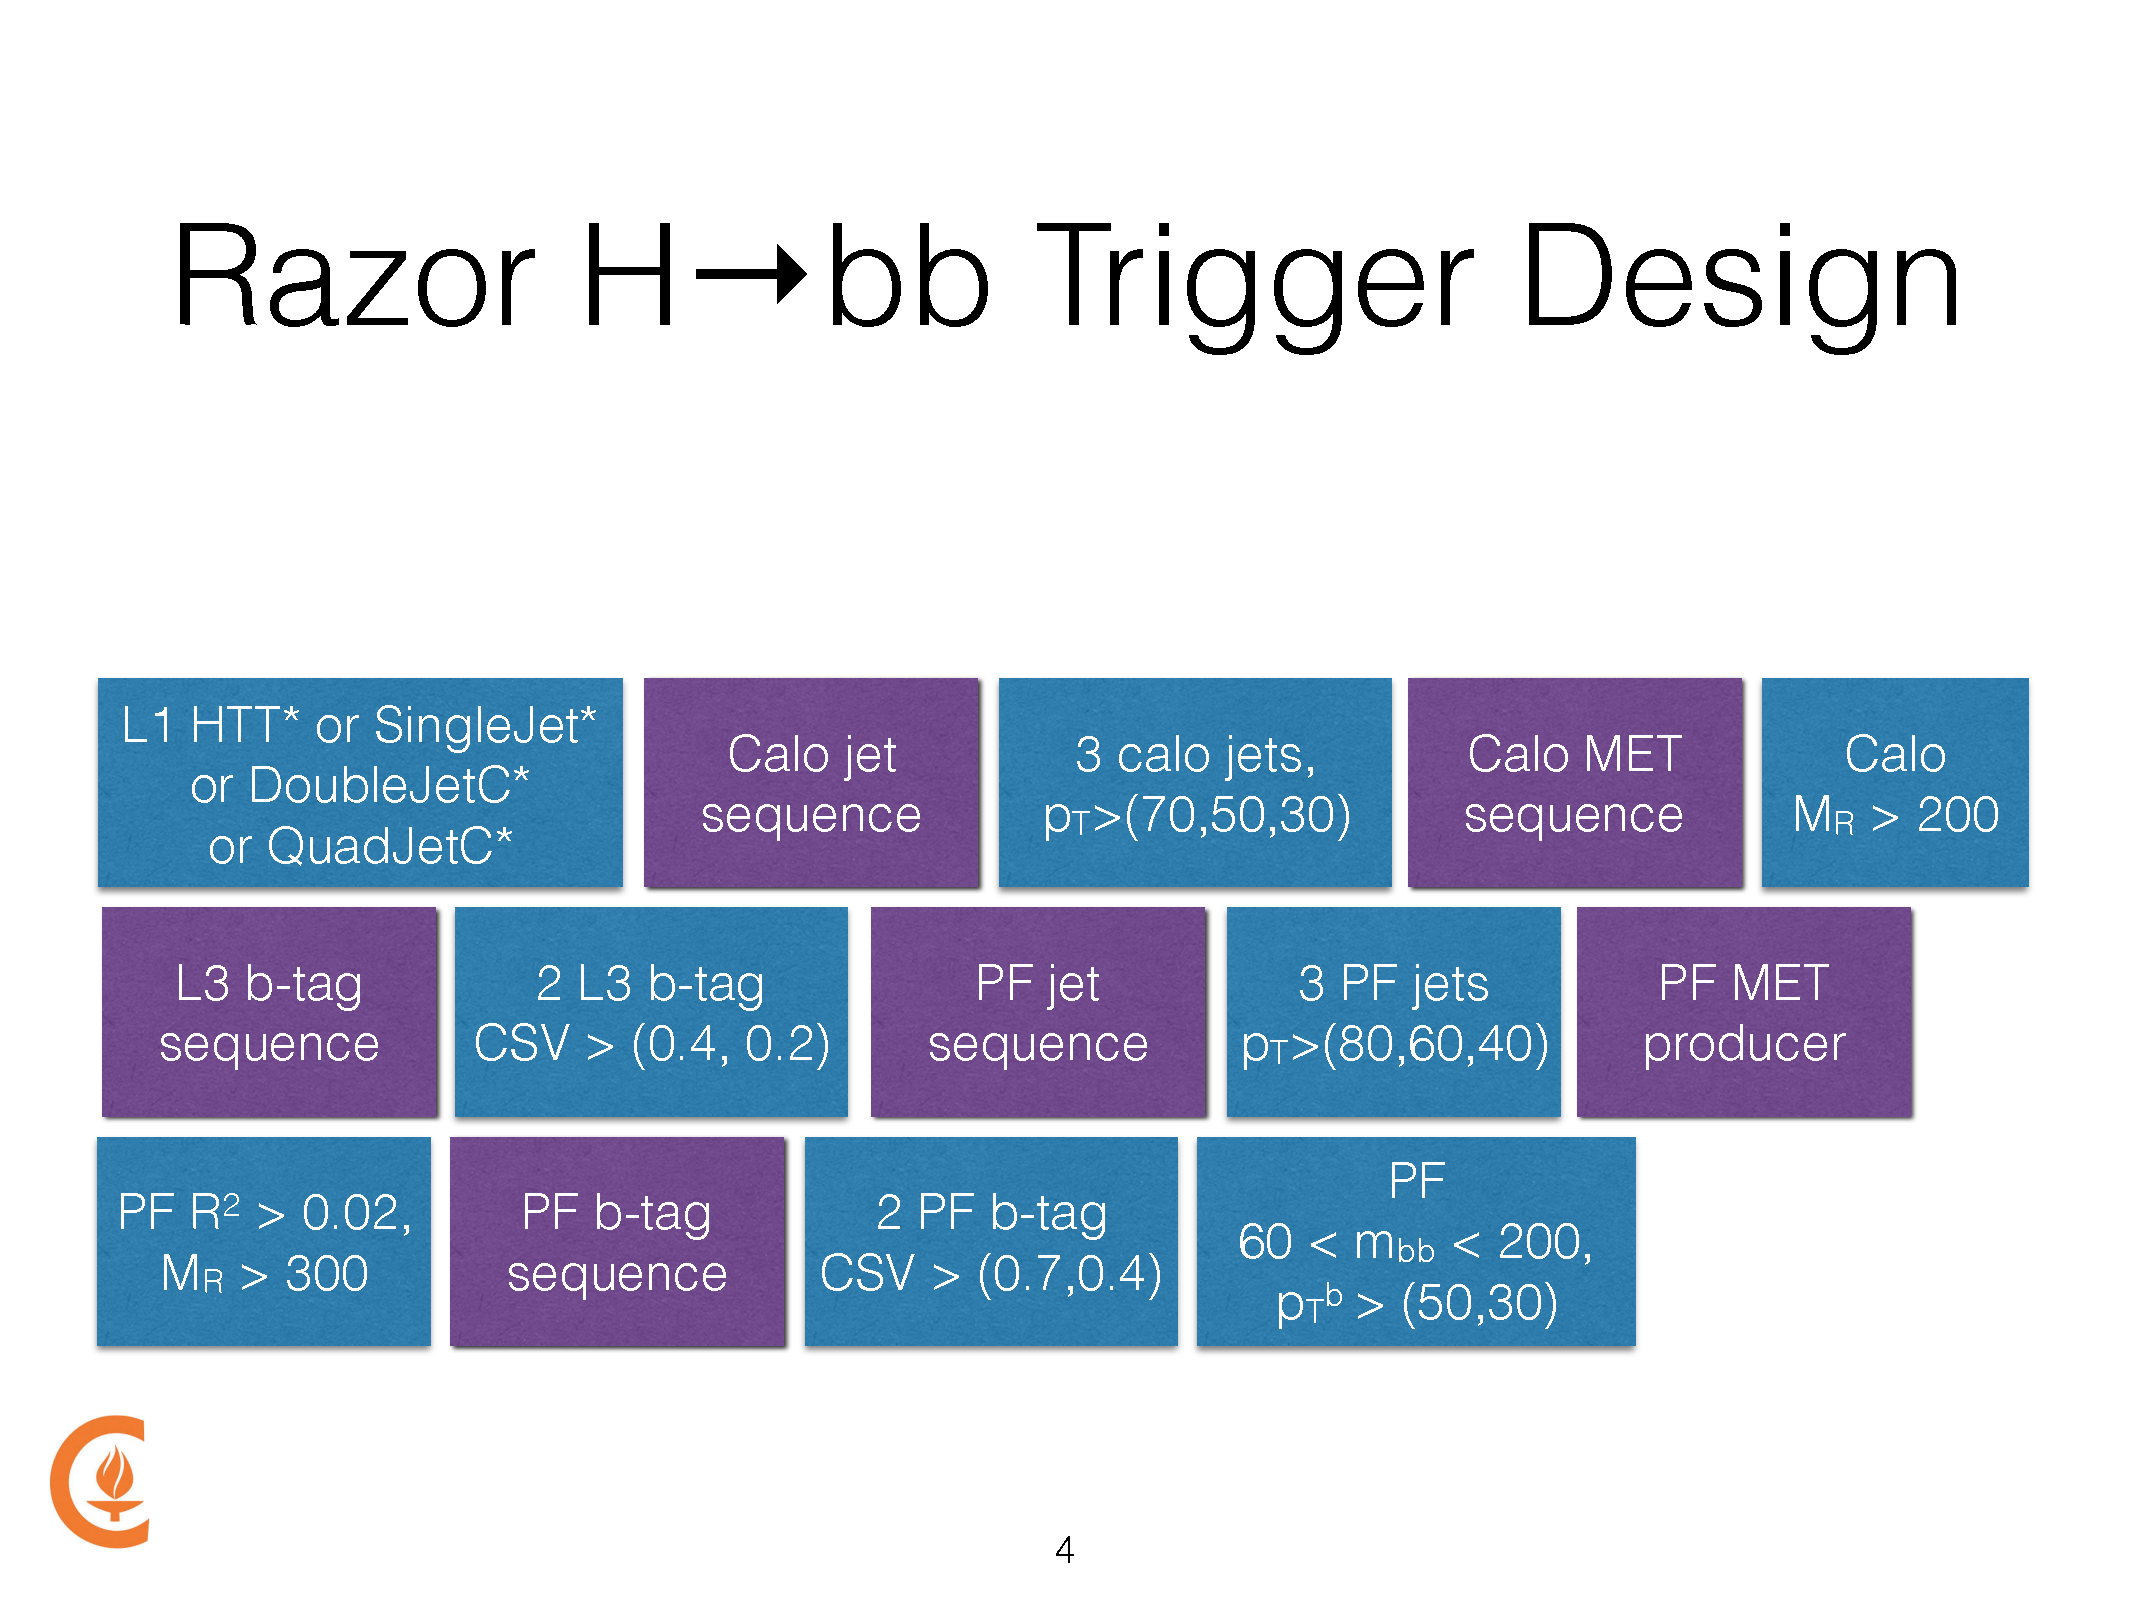
\includegraphics[width=0.8\textwidth,clip=true,viewport=0 110 1024
500]{figs/hlt13TeV/HLTRazorHbbDesign.pdf}\\
(d) HLT\_Rsq0p02\_MR300\_TriPFJet80\_60\_40\_\\
~DoublePFBTagCSV0p7\_0p4\_Mbb60\_200
\caption{\label{fig:HLTdesign} Flow of the producer steps (in purple)
  and filter steps (in blue) in
  the razor triggers.}
\end{figure}

\section{HLT Rate and Average CPU Time}

The HLT rates and average CPU time consumed for the razor triggers, as measured in data
collected in 2015, are presented in Tab.~\ref{tab:rates2015}.

%\begin{table*}[ht!]
%\centering
% \caption{Rates for 0\unit{T} triggers.
% \label{tab:rates0T}}
%\resizebox{\textwidth}{!}{
%\begin{tabular}{l|l|l}
%\multirow{2}{*}{Trigger path} &  Data rate (run 260039) & MC rate (Spring '15) \\
% &  $4\times 10^{33}$ \unit{cm$^{-2}$ s$^{-1}$}, 17 PU &  \\\hline
%HLT\_Rsq0p25\_Calo & 3.7 Hz & \\
%HLT\_RsqMR240\_Rsq0p09\_MR200\_4jet\_Calo & 5.6 Hz & \\
%HLT\_RsqMR240\_Rsq0p09\_MR200\_Calo & 18.2 Hz & 
%\end{tabular}}
%\end{table*}

\begin{table*}[ht!]
\centering
 \caption{HLT rates and average CPU time consumed for the razor
   triggers under different running conditions in 2015. Run 260627 had peak $5\times 10^{33}$ cm$^{-2}$
   s$^{-1}$ peak instantaneous luminosity with 17 average pileup
   interactions, while run 259721 had $1.5\times 10^{33}$ cm$^{-2}$
   s$^{-1}$ peak instananeous luminosity with 23 average pileup interactions. \label{tab:rates2015}}
\resizebox{\textwidth}{!}{
\begin{tabular}{l|l|l}
\multirow{2}{*}{Trigger path} &  Data rate (run 260627) & CPU time (run 259721) \\
 &  $5\times 10^{33}$ cm$^{-2}$ s$^{-1}$, 17 PU &  $1.5\times 10^{33}$ cm$^{-2}$ s$^{-1}$, 23 PU \\\hline
HLT\_RsqMR240\_Rsq0p09\_MR200 & 7.7 Hz & 27 \unit{ms}\\ 
HLT\_RsqMR270\_Rsq0p09\_MR200 & 2.3 Hz & 17 \unit{ms} \\ 
HLT\_RsqMR240\_Rsq0p09\_MR200\_4jet & 1.2 Hz & 20 \unit{ms}\\
HLT\_RsqMR270\_Rsq0p09\_MR200\_4jet & 0.5 Hz  & 15 \unit{ms} \\
HLT\_Rsq0p25 & 0.7 Hz & 14 \unit{ms}\\
HLT\_Rsq0p30 & 0.4 Hz & 14 \unit{ms} \\
HLT\_Rsq0p02\_MR300\_TriPFJet80\_60\_40\_&\multirow{2}{*}{16.0 \unit{Hz}} & \multirow{2}{*}{34 \unit{ms}}\\
~DoublePFBTagCSV0p7\_0p4\_Mbb60\_200 & &\\
HLT\_Rsq0p02\_MR300\_TriPFJet80\_60\_40\_ & \multirow{2}{*}{8.0 Hz} & \multirow{2}{*}{26 \unit{ms}}\\
~DoublePFBTagCSV0p7\_Mbb60\_200 & & 
\end{tabular}}
\end{table*}
% timing from: 
% https://docs.google.com/spreadsheets/d/1qu0dKZfjHEl073QyXayxzPBNoT10GZKMiPU9-z8VSeU/edit#gid=0
% supplemented by my measurement (for RsqMR240...)
% https://www.dropbox.com/s/z8qfx57du7h3gzq/TSG_RazorHLT2016_30Mar2016.pdf?dl=0


\section{Pileup Dependence}

The HLT rate, normalized by the number of collinding bunches, as a function of the number of pileup interactions for
each razor trigger and for different data runs collected in 2015 is
shown in Fig.~\ref{fig:HLTpileup}. Nominally, the dependence of the
normalized HLT rate on pileup is expected to be linear, as is the case
for single-object triggers. Contrastingly, triggers based on``sum'' quantities
(such as $H_\mathrm{T}$ or $\MET$) and multi-object triggers often
demonstrate a nonlinear dependence on pileup~\cite{Bocci:2016}. As the
razor triggers are both based on sum quantities and multiple objects,
they also exhibit some nonlinear dependence on pileup. This implies
that as the pileup increases at the LHC in 2016 and beyond, either trigger thresholds
will need to rise dramatically or more sophisticated methods to deal
with pileup contamination will need to implemented. One such method is
delineated in Ch.~\ref{ch:timing}.

\begin{figure}[ht!]
\begin{tabular}{cc}
\centering 
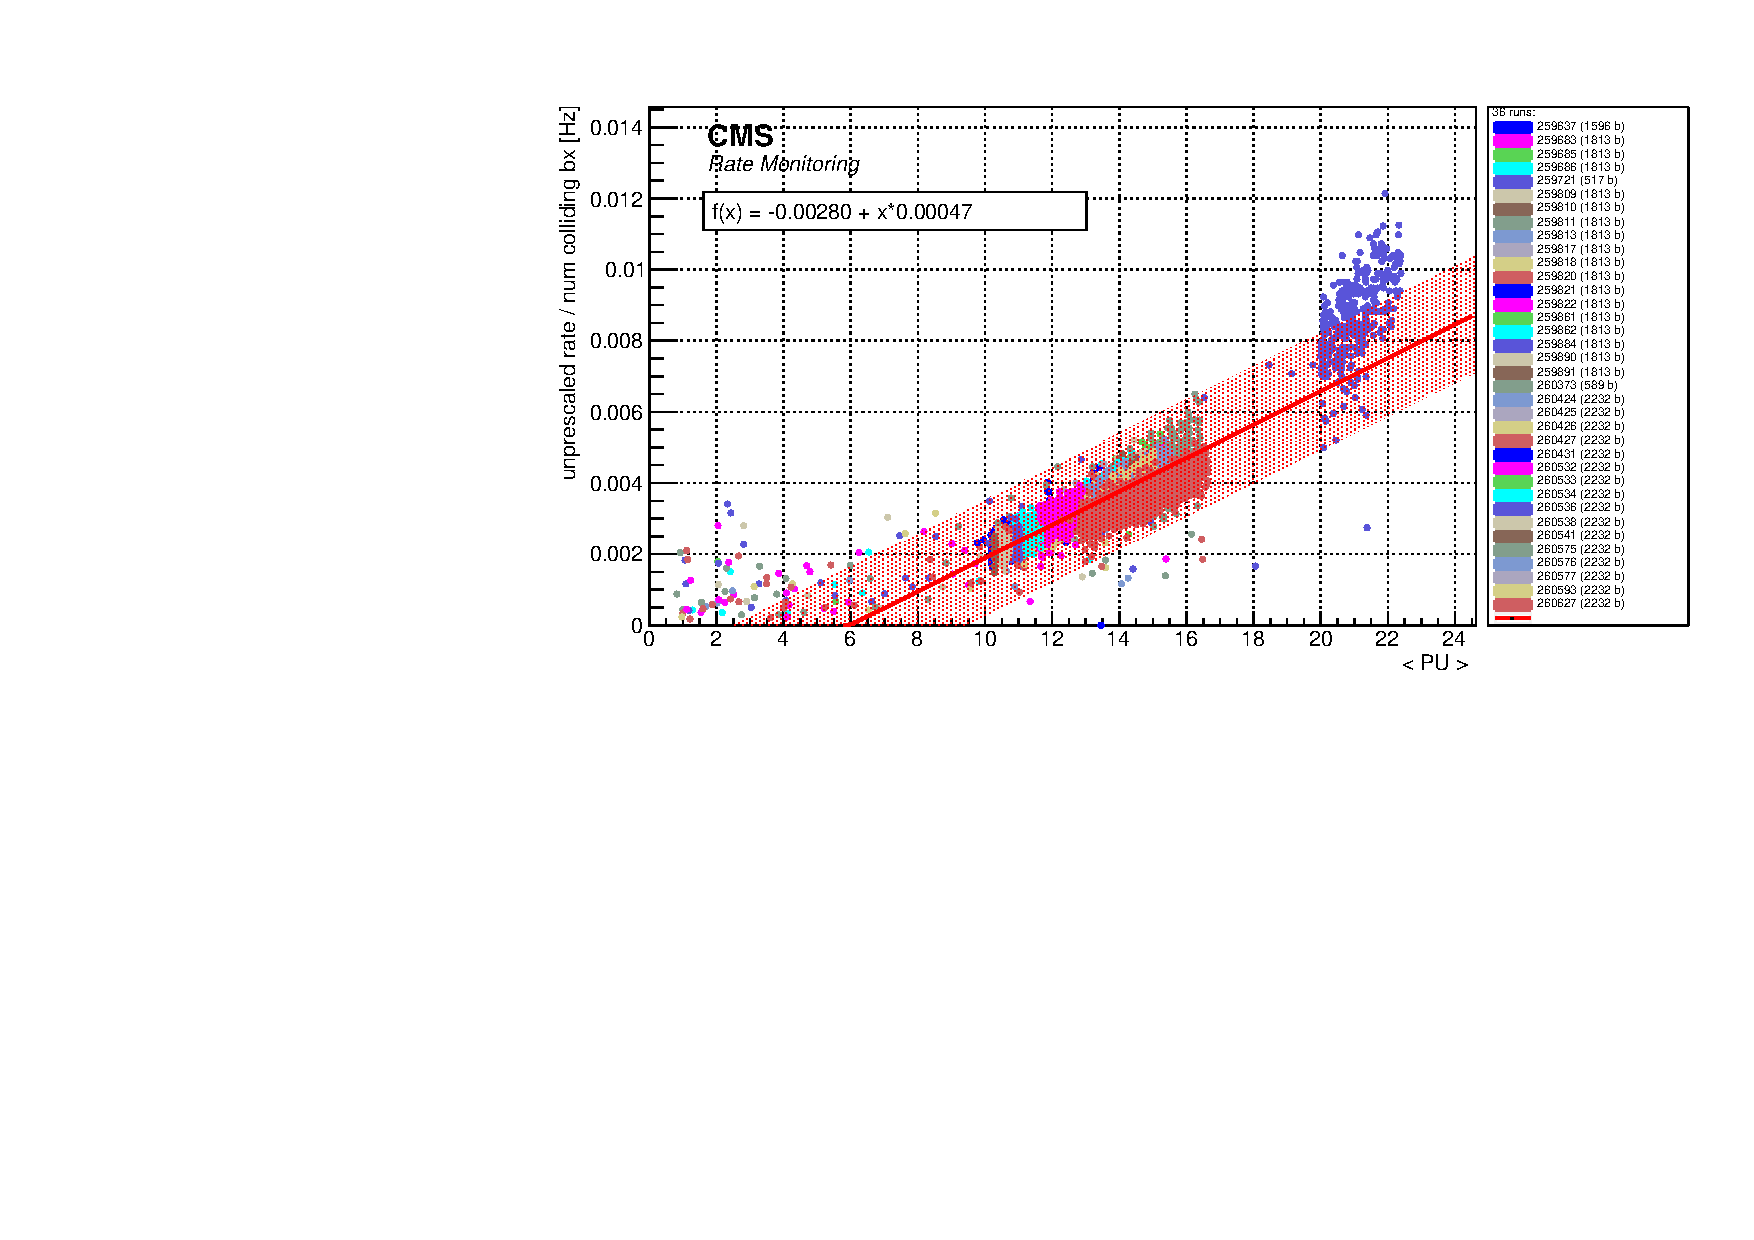
\includegraphics[width=0.49\textwidth]{figs/hlt13TeV/linear/HLT_RsqMR240_Rsq0p09_MR200_instLumi_vs_rawRate.pdf}
  & 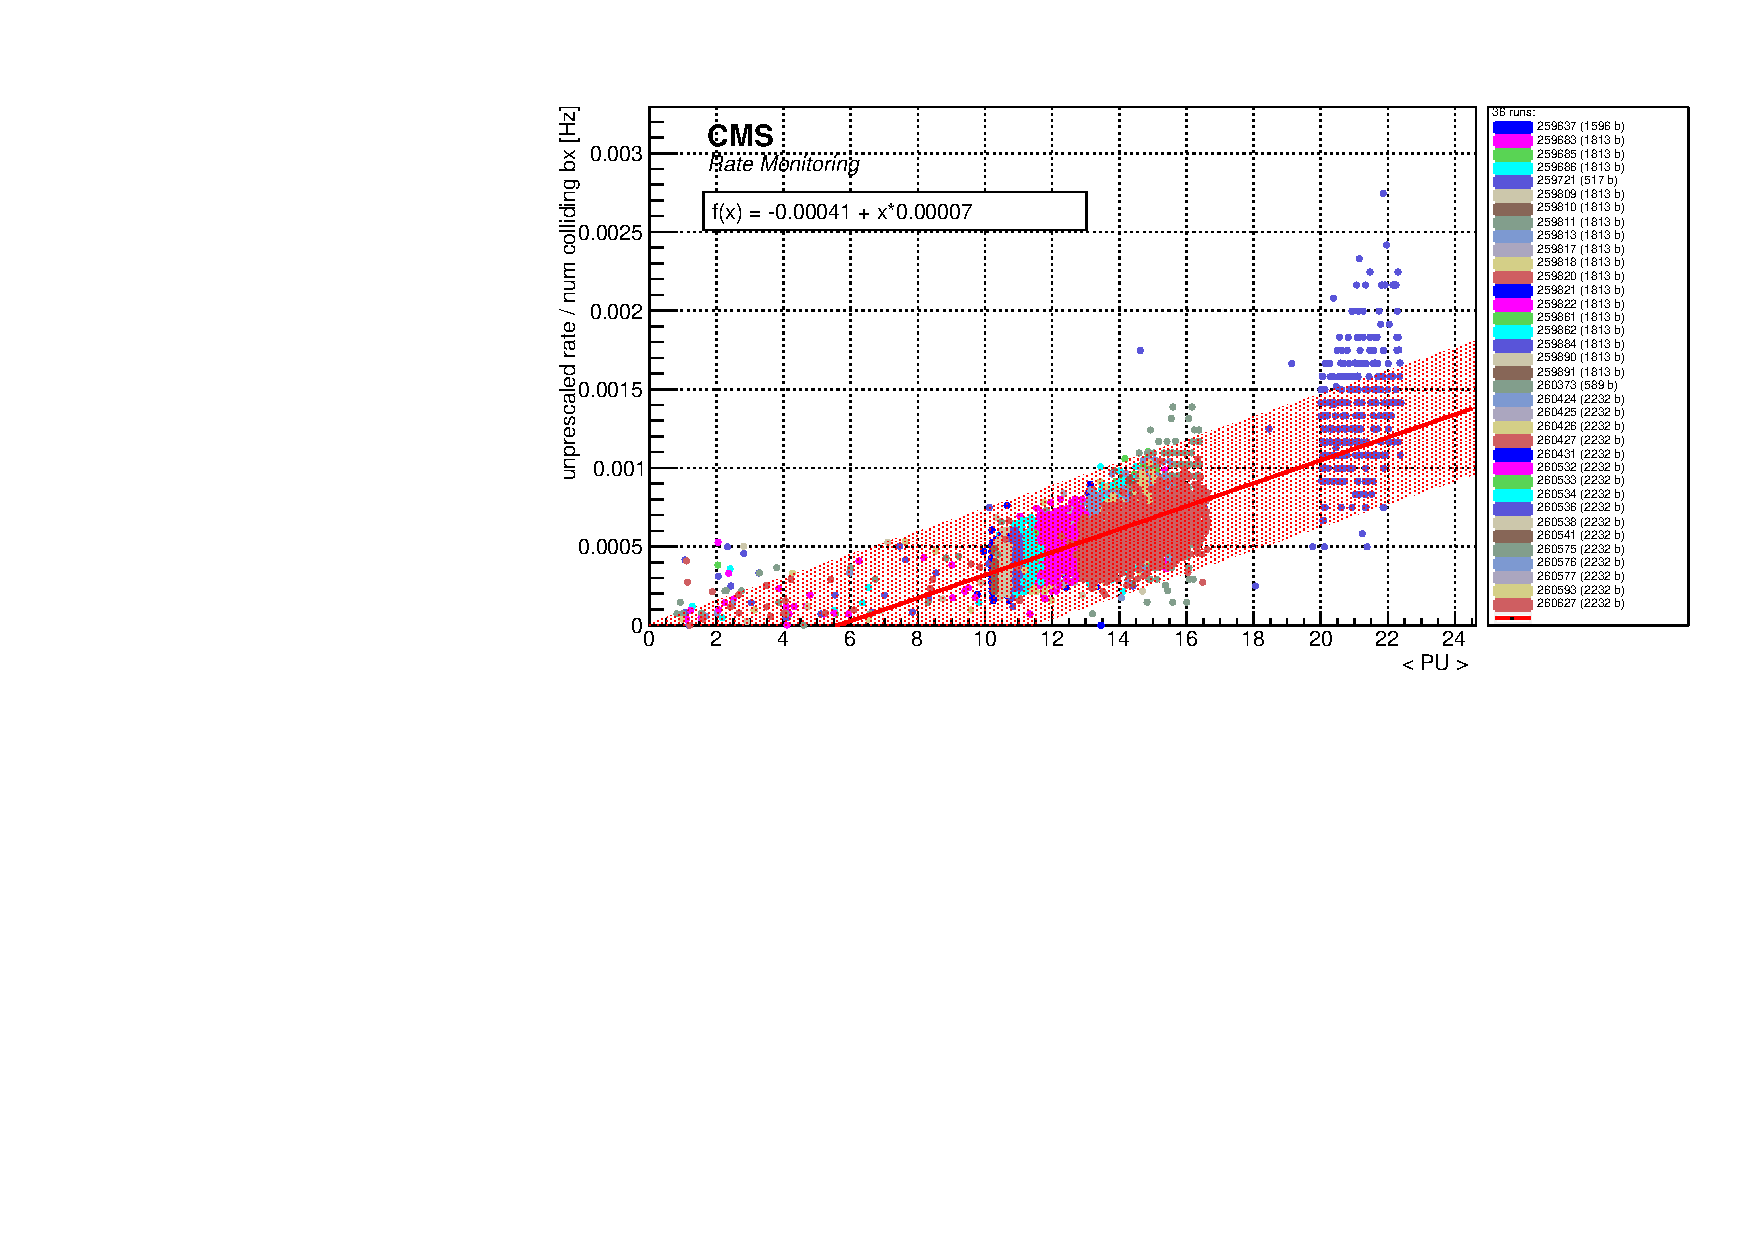
\includegraphics[width=0.49\textwidth]{figs/hlt13TeV/linear/HLT_RsqMR240_Rsq0p09_MR200_4jet_instLumi_vs_rawRate.pdf}\\
(a) HLT\_RsqMR240\_Rsq0p09\_MR200 & (b) HLT\_RsqMR240\_Rsq0p09\_MR200\_4jet\\
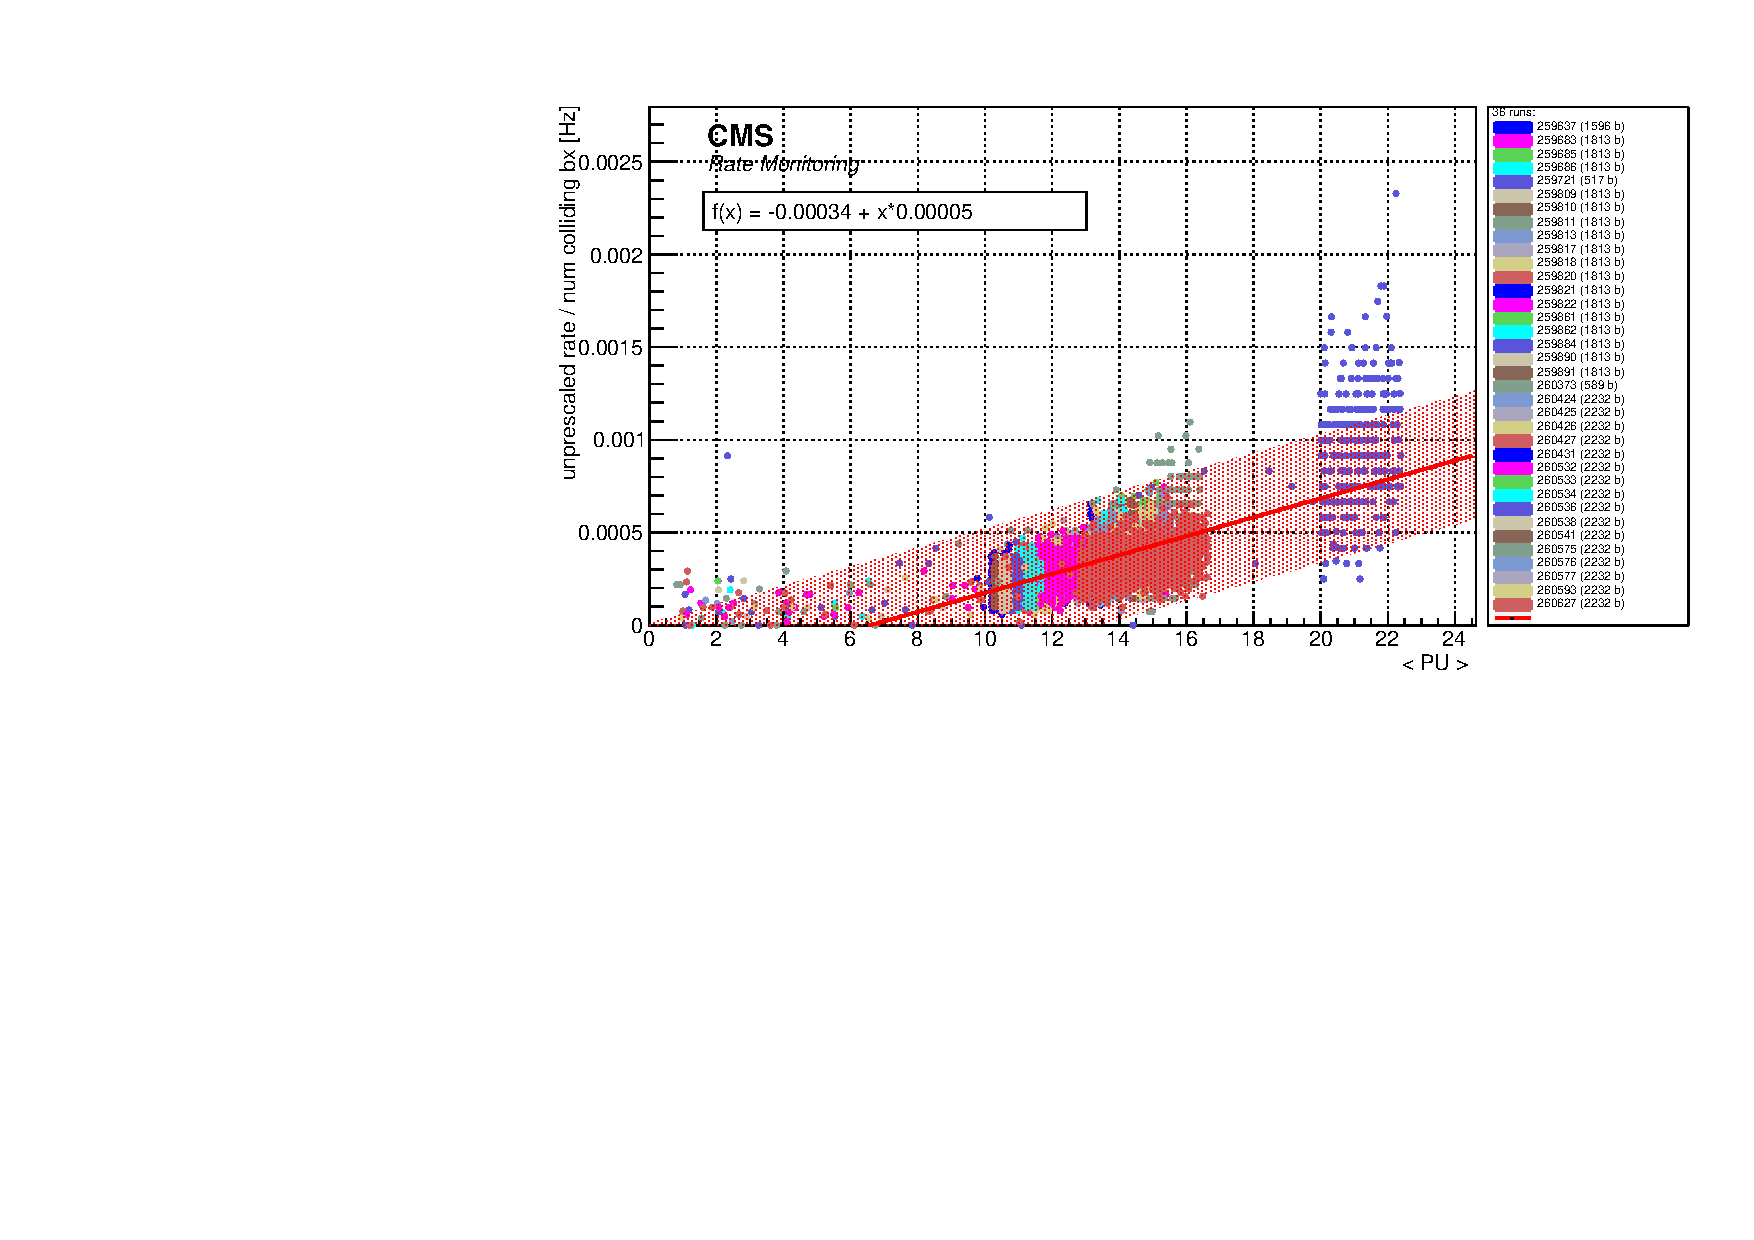
\includegraphics[width=0.49\textwidth]{figs/hlt13TeV/linear/HLT_Rsq0p25_instLumi_vs_rawRate.pdf}
  &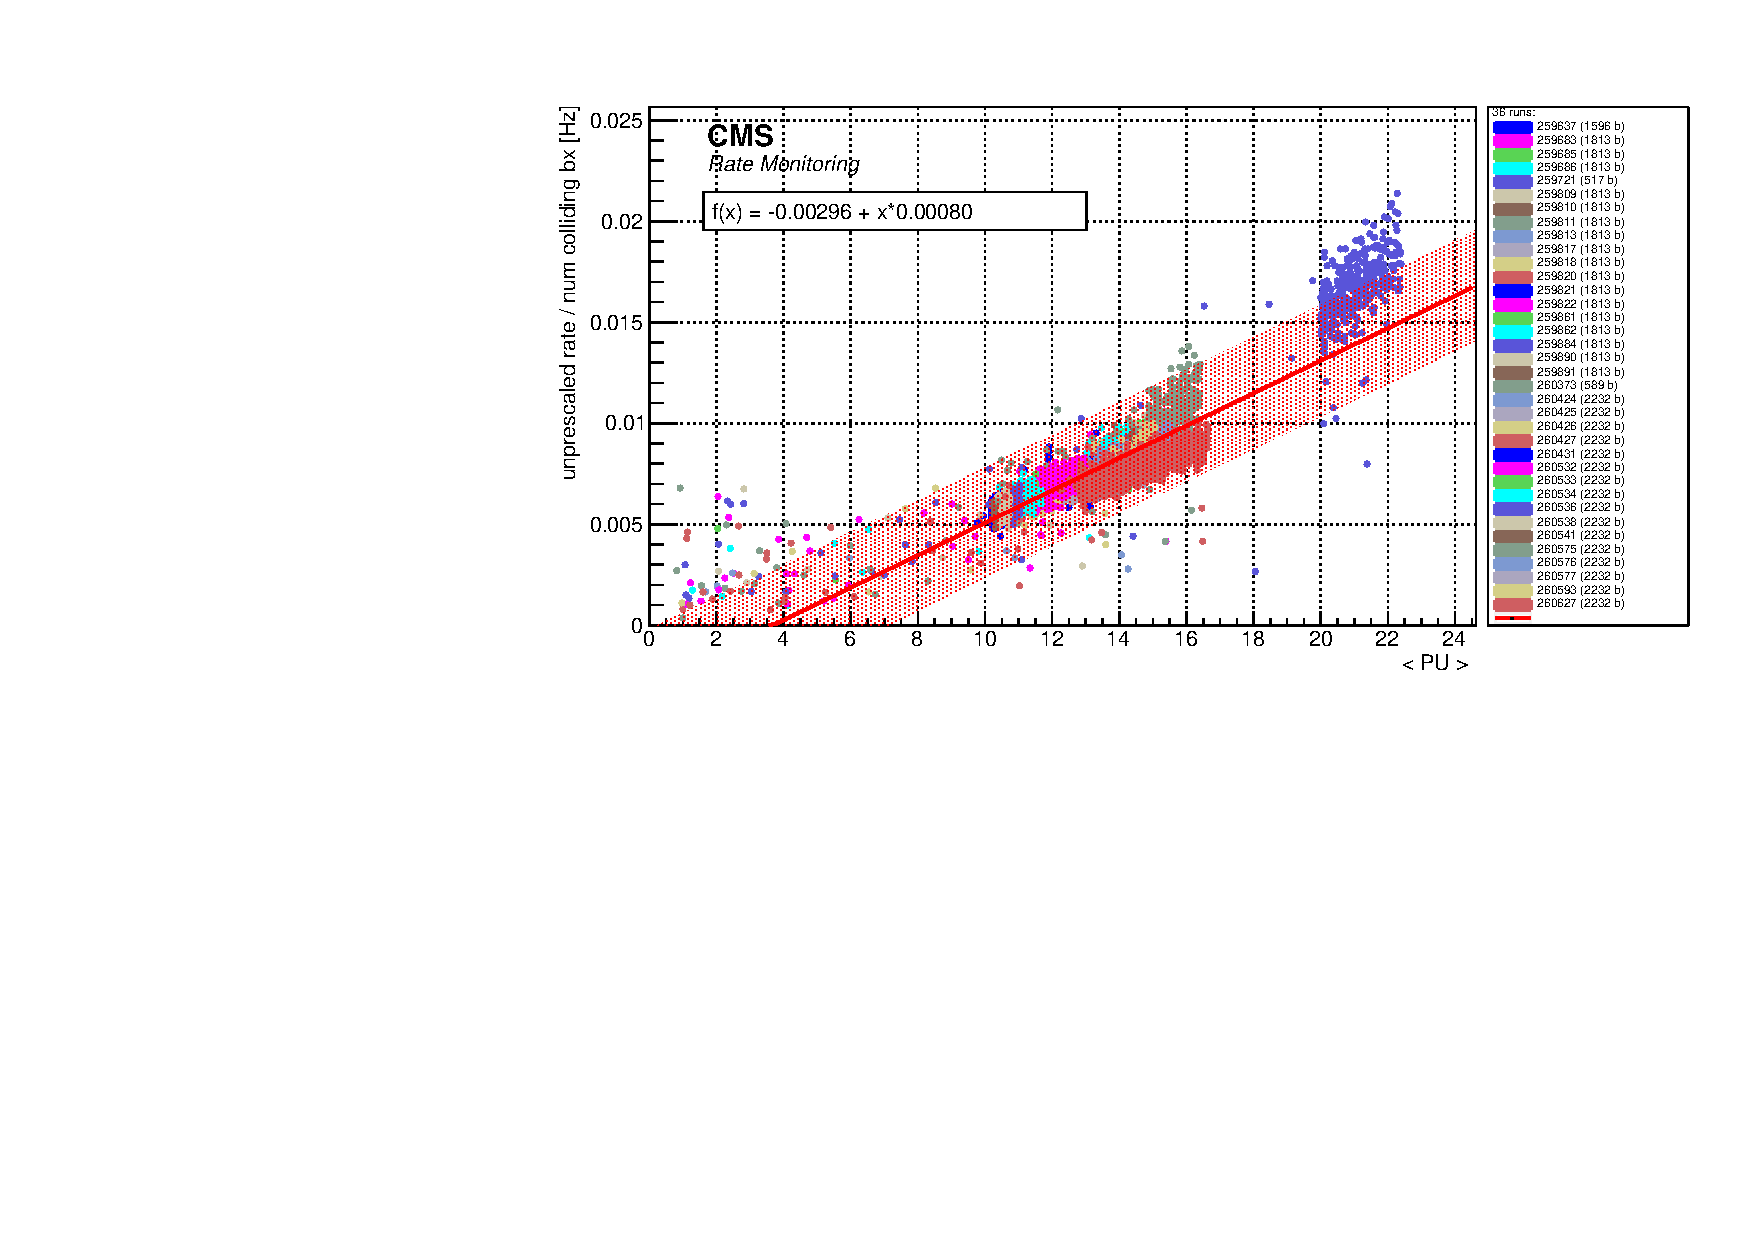
\includegraphics[width=0.49\textwidth]{figs/hlt13TeV/linear/HLT_Rsq0p02_MR300_TriPFJet80_60_40_DoublePFBTagCSV0p7_0p4_Mbb60_200_instLumi_vs_rawRate.pdf}\\
\multirow{2}{*}{(c) HLT\_Rsq0p25} & (d) HLT\_Rsq0p02\_MR300\_TriPFJet80\_60\_40\_\\
& ~DoublePFBTagCSV0p7\_0p4\_Mbb60\_200
\end{tabular}
\caption{\label{fig:HLTpileup} Pileup dependence of the razor triggers.}
\end{figure}


